\chapter{Configuration and testing}
\label{configurationandtesting}
\todo{differentiate betwee simulation and navigation 2 chapters?}

This chapter will contain the configuration of all nodes of the concept. In addition the newly developed nodes have to be tested as well as the entire navigation concept.

The nodes of the system are highly interconnected, therefore it is hard to test nodes while eliminating the error of others.

The final config of the discussed nodes can be found in Appendix \ref{config}.

\section{URDF and robot\_state\_publisher}

The URDF model is based on the model of Christen Lofland, who created this for his own open source project\cite{chrisl8}.\\

Unfortunately this model has been created to generate the fixed transforms of a real model only, so it does not have moveable joints for the wheels or any plugins for sensors and the differential steering. In addition to that it uses .stl files for both visual and collision volumes which results in unpredictable collision distances.\\

To keep the model as simple as possible one common xacro file is used, that loads the individual files for the following parts:
\begin{itemize}
	\item Arlo body
	\item Camera
	\item Lidar
	\item IMU
	\item Gazebo plugins for all sensors and differential drive
\end{itemize}

All of the files are Xacro files in contrast to pure URDF so parameters and macros can be used, which makes the robot model more flexible.\\

The plugins for Gazebo have not been included in the individual files so the URDF can be used for real robots with a similar sensor setup without big modification but just with the exclusion of the plugin file.

The resulting robot then looks like pictured in Figure \ref{arlourdf}.

\begin{figure}[H]
	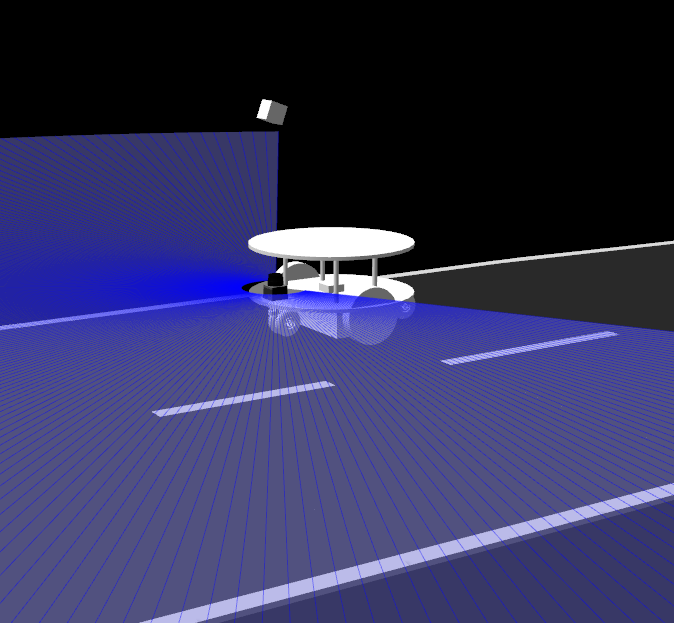
\includegraphics[width=\textwidth]{Pictures/arlourdf}
	\caption{ArloBot URDF with sensors and Gazebo plugins}
	\label{arlourdf}
\end{figure}


Using rqt\_tf\_tree the tf tree can be checked for conformity to ``REP 105'' and the concept.\\ 
The tf\_tree of the running concept is pictured in Appendix \ref{config}.\\
As visible the fixed frame of the setup is ``map'' the following transform to the ``odom'' frame is published by cartographer. The transformation between the ``odom'' frame and ``base\_footprint'' then gets published by robot\_localization here named ``ekf\_se''.\\
The following transformations and frames are published by ``robot\_state\_publisher'' according to the URDF of the robot.

\section{Gazebo}
The setup of the simulation consist out of the modeling of the world, the conversion of the model into a sdf file and the general launch file.

As described in the concept the world will be modeled using the software blender.\\

The modeling itself is very straight forward since one segment of the road can be modeled and extruded along a closed path like pictured in \ref{simworld}. 

The course of this road has been constructed to feature the following elements:

\begin{itemize}
	\item Left and right curves
	\item Tight and wide curves
	\item Long straight section
\end{itemize}

It will be the environment for most of the following tests.

\begin{figure}
	\centering
	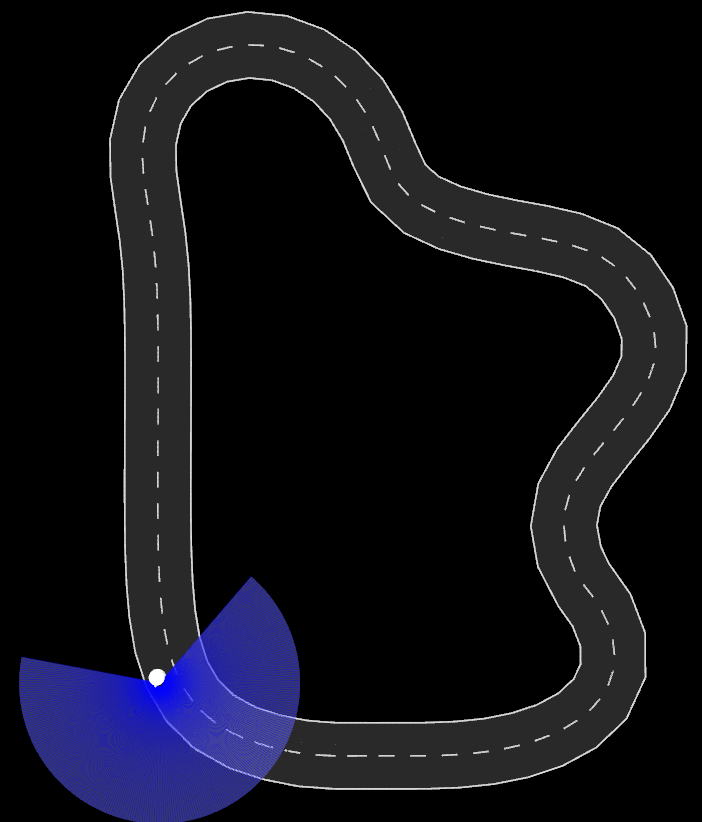
\includegraphics[width=.5\textwidth]{Pictures/test track}
	\caption{finished simulation world used for various tests}
	\label{simworld}
\end{figure}

Gazebo then can be started from a launch file by defining the generated world.\\

\subsection{Plugins}
The configuration of the sensor and drive plugins are fairly straight forward, based on the tutorial page in the Gazebo documentation\cite{gazebotutorial}.\\



While trying to simulate the original camera of the robot based on its datasheets (Appendix \ref{AppendixDataSheets}) and the calibration parameters, it is observable that not all parameters of the camera\_info message can be set in the sdf description of the plugin.

Overall it does not seem to be possible to mimic the original camera, hence the camera will be modeled without distortion with the assumption that a calibrated camera and image rectification packages like ``image\_proc'' would produce a comparable result.






\section{road\_detection}
The road\_detection provided by Prof. Dr. Stefan Hörmann consist out of the following six nodes of which some need configuration to work with the specific camera setup.

\begin{itemize}
	\item edgeDetector
	\item edgeProjector
	\item LineFinder
	\item LineTracker
	\item RoadDetector
	\item RoadRecordEvaluation
\end{itemize}

The edgeDetector is the first node of the package and extracts the edges from the picture using canny filters. Here the expected line width in pixels has to be configured. The easiest way to determine the width is to run the node and take a look at the picture published on the topic ``/roadDetection/image\_edges''. Then rqt\_reconfigure can be used to raise the maxLineWidth parameter, until the entire line of the road is visible in the filtered picture. In the case of the simulation the adjustment of the canny thresholds is not required, since the environment has only black and white colors and no greyscale.\\

The edgeProjector has the task to project the image on the 2D surface and therefore must know the position and orientation of the camera relative to the ground. While doing so it rectifies the image according to the provided camera information, which should contain the calibration parameters of the setup.

To get a reliable result from the ``LineFinder'' the amount of tiles in x and y has been increased to get more precise lines from the internally used hough transformation.\\
In this scenario the robot drives on a wider road than usual for the Carolo-Cup, so the parameter maxSegmentDistance has been increased to 0.9 m so the line segments of the middle line will still be matched to the same line.\\
When the robot drives around a tight corner the road often starts at an angle relative to the robots x axis. The parameter ``maxStartAngleDiff'' has been increased to 75° to get more coverage in this case.\\

While configuring the road detection the first step is to configure the orientation and position of the camera in the node``edgeProjector'' according to the definition in the URDF file. In addition to that the camera picture has to be cropped so the robot is not visible anymore in the picture.\\

In the ``LineTracker'' node the distance, at which lines should be evaluated needs to be set, so the node does not see the edge of the picture, in which the distortion has the largest effect.\\


The RoadDetector node needs an estimate for the lane width as a min and max value and a maximum angle between two individual road markings. These values are obviously specific for the environment.\\

\section{MarkFreeSpace}

The parameters in Table \ref{markfreespaceparams} have to be configured so the robot will have a tendency to the right lane but still is able to drive on the left lane, if necessary. This means, that the maxcost has to be significantly smaller than the lethal (254). The Minimum cost has to be smaller than the neutral cost of the global planner, which defaults to 50. To complicate the transition to the left lane, the inflation radius of it is set to 50\% of the right lane and the radius of the right cost removal  is set to 40\% to guarantee a free space on the right road side.\\
Around obstacles the cost removal is set to 1.5 meter so the obstacle avoidance will finish within the 2 meter guideline defined in the Carolo-Cup rules\cite{carolocup}.\\

The distances between the inflated points and the cleared points has to be fairly large to limit the computational load. For the inflation only the last point of the polynomial will be inflated, since a uniform cost distribution along the road marking is not too important. The distance between the cleared cells is set to 0.5 meters, to guarantee a clear section on the right lane.

The final configuration is pictured in Appendix \ref{config}.


\section{Cartographer}
The goal of this node is to produce a map that gets more reliable over time.\\

Unfortunately the data available for Cartographer is very self similar, meaning a straight road will always look the same and therefore does not have sufficient features for proper loop closure. In contrast to the points from the road detection the lidar can actually supply such features and will therefore be a good improvement for the resulting map.\\

But it is not guaranteed that the lidar will even sees anything the SLAM algorithm has to work with the points of the road detection only as well.\\

The basic configuration of Cartographer is purely based on the setup of the robot. In this case Cartographer is supposed to use lidar and the points of the road detection at the same time. To reduce the amount of times one of the sensor doesn't see anything, these will need to be merged in the markfreespace node and Cartographer will receive one PointCloud2 only.\\
To improve the map further the odometry supplied by the robot\_localization package is used as an input, as well as the IMU.

Furthermore Cartographer will be set to 2d map building.


\subsection{Tuning}
With the basic configuration of Cartographer is not able to provide a reliable map and a tuning procedure has to be performed. Here the general recommendation of the tuning guide should be followed, which states to tune local SLAM first and disabling global slam while doing so \cite{cartographertuning}.
To tune the local SLAM the parameter of the tracjectory builder have to be adjusted.\\
The trajectory builder contains a scan-matcher, which will compare incoming sensor data and tries to align it with each other as good as possible. This behavior can be tuned by configuring the size of the linear and angular search windows and the weight for the rotation and translation of the incoming scans.\\
One more important setting is the size of the sub maps. These can be adjusted by the amount of scans they contain. Since the submaps will consist out of the scan matched obstacles it is important to set the size of the submaps not to high, if the incoming data will be very self similar. Otherwise the scanmatcher will combine too many scans while shifting them over each other since they look so similar. This results in both rotational and translational error.\\
As soon as the local SLAM produces a reliable result after multiple rounds of the robot the global SLAM can be activated and tuned.\\

The global SLAM has two options of combining the submaps the loop-closure, which will check, if the robot was at this spot already, and a scanmatcher, which will try to match the submaps to the current scan. For both of these the weights can be adjusted individually and like in the local SLAM the size of the window for translation and rotation can be adjusted. Reducing the window size to a minimum is important when dealing with self similar data, so the submaps will not be shifted on top of each other. The size should be chosen so the global SLAM can still correct errors of the individual submaps.\\
With these values and the submaps the global planner calculates constraints between the maps which will be valued between 0 and 1. These constraints can be blocked with a threshold value that will block constraints with a smaller value. Like this the computation time can be drastically reduced and only the important constraints will be processed. Furthermore the weighting of the pose of the odometry and the local SLAM can be adjusted, which can be useful with bad odometry.

\subsection{Testing}
Testing of the SLAM will mostly consist out of a Black-Box test meaning the only things that will be observed is the output and therefore the map.
The SLAM will be tested in the following cases:
\begin{itemize}
	\item Data purely from the road detection.
	\item Data from road detection and lidar scan with obstacles on the side of the road.
	\item Long duration test with both road detection and lidar scan with obstacles on the side of the road.
	\item Data from road detection and lidar scan with obstacles on the road.
\end{itemize}

During all of these tests the navigation will solely work with the predicted goals since it is yet unsure if the SLAM map is even usable. Furthermore the same tuning will be used for all tests.\\



\section{PoseFinder}

Starting with the goal extraction from the map, the parameter ``MapCostThresh'' will be set to 50, meaning the probability of being an obstacle has to be at least 50\%. The reduction radius has to be configured slightly larger than the road width, so the points extracted on both road markings can be combined, even if the road is slightly angled. With a road width of 1.8 meter, 2 meter will be chosen for this parameter.\\

The parameter ``GoalDist'' has to be configured smaller, that half of the costmap width so it can be guaranteed, that the goal is all ways located inside the bounds of the costmap to prevent errors. With a costmap width and hight of 9 meter the parameter is set to 4 meter.\\

To switch between the circle and line approximation the parameter ``CRadThresh'' is set to 6m. Setting this parameter higher will improve the performance in wide turns while the performance on straight sections will get worse and vice versa.\\

Finally the GoalAngle for the circle approximation has to be configured. This is set to $0.3\pi$, meaning the window of trustworthiness of the circles is 60°.




\section{Costmaps}
Based on the fact that both planners are responsible for different tasks the configuration of the individual costmaps need to fulfill different tasks too. The requirements of the two planners will be compared in order to determine the configuration of their individual costmap.\\

As described in the theoretical knowledge of this thesis the costmap are structured in layers. This means that the data can be evaluated by different plugins before it will be combined into the real costmap.\\

It makes sense to first take a look at the general behaviour, that both planners share. In this case it is obstacle avoidance. This means that the lethal obstacles need to be marked in both costmaps.\\

To implement this the provided plugin obstacle\_layer can be used. It will take incoming sensor data (sensor\_msgs::PointCloud or sensor\_msgs::LaserScan) and mark the points in the costmap.\\

Since the data here comes form the road detection and a lidar and both have a certain resolution it is unsure, if the result of a scanned obstacle in the costmap is actually a closed line or just points, since this highly relies on the resolution of the sensors and the costmap.\\

To fill theses gaps in the costmap the provided plugin inflation\_layer can be used. It will inflate only the lethal obstacles in the costmap with a configurable cost distribution.\\

This setup is already enough for the local costmap, where as the global planner needs to fulfill the quest of changing lanes if necessary but always preferring the right lane. For this a custom plugin will be needed that makes the transition to the left lane more expensive but still possible.


The final layer plugin setup of the costmaps results in the following:\\

\textbf{Global costmap:}
\begin{itemize}
	\item obstacle\_layer
	\item inflation\_layer
	\item dynamic\_cost\_layer
\end{itemize}


\textbf{Local costmap:}
\begin{itemize}
	\item obstacle\_layer
	\item inflation\_layer
\end{itemize}

The costmaps will both have the same size that should always be larger than the distance, at which the goalfinder searches for goals.

Since both costmaps are rolling window costmaps they will reference the continuos frame ``odom'' and move with the frame ``base\_footprint''.

Counterintuitively the robot radius needs to be set smaller than the robot actually is. Otherwise the slightly moving obstacles collide with the footprint and the global planner can not produce a valid path that the local planner can follow.\\
This footprint is only considered by the global planner, which is only required to provide a rough path. The local planner has its own setting for a footprint, therefore the obstacle avoidance will still work as expected.

The last remaining settings are the resolutions and the frequencies of the costmaps, which are chosen based on the performance of the navigation and the computational load.


\section{Planners}

\subsection{global\_planner}
\label{globalplannertest}
There is not much room for configuration, when it comes to the global\_planner of the navigation\_stack. Probably the most important step for computation load is the choice of a planning algorithm.\\
The two algorithms that are offered by the global\_planner node are Dijkstra and A*.\\

\begin{figure}[H]
	\begin{subfigure}{.5\linewidth}
		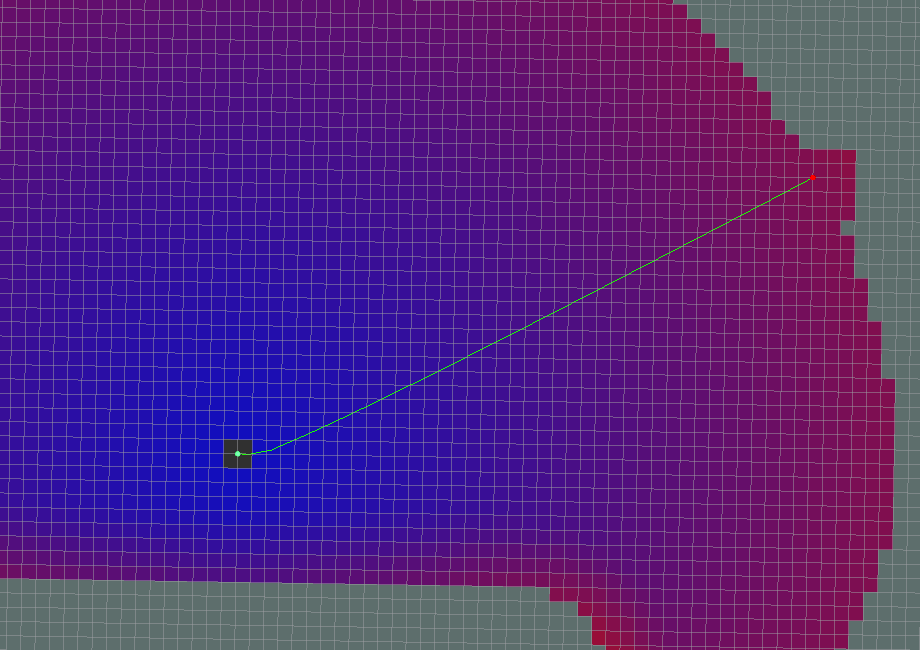
\includegraphics[width=\textwidth]{Pictures/Dijkstra}
		\caption{Dijkstra}
	\end{subfigure}	
	%\hskip2em
	\begin{subfigure}{.5\linewidth}
		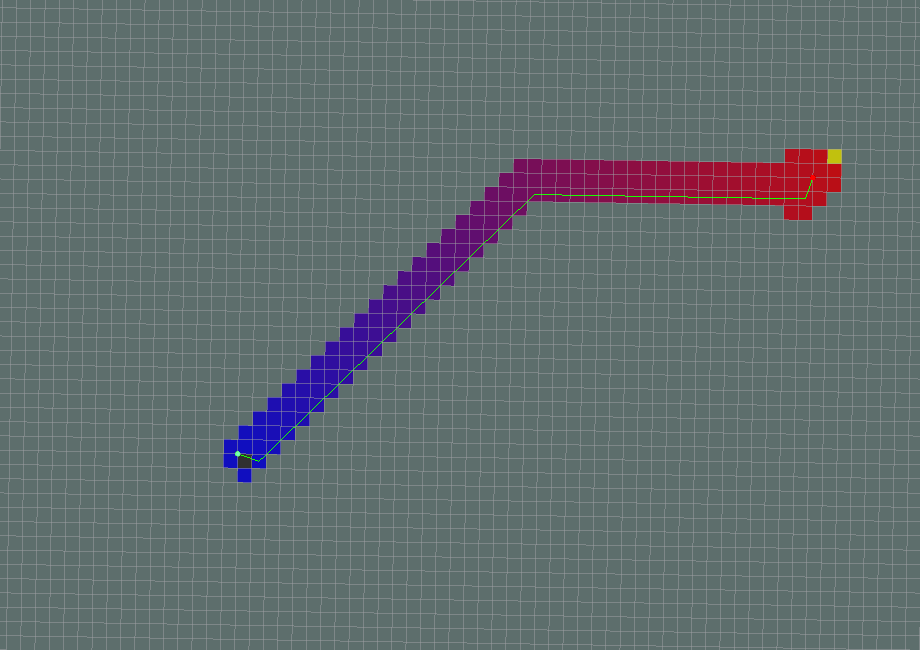
\includegraphics[width=\textwidth]{Pictures/AStar2}
		\caption{A*}
	\end{subfigure}

	\caption{planning algorithm comparison (grey cells are not observed)\cite{globalplanner}}
	\label{plannercomparison}

\end{figure}


It is obvious, that A* is much more efficient in this use case since the robot will mostly go straight or in a slight curve. Therefore A* will be chosen for the global planner.\\

Another important setting is necessary since the global costmap is used as a rolling window costmap. The global\_planner will be default outline the global costmap with lethal cost to prevent the global planner to plan outside of a fixed costmap. This behaviour results in artifacts, after the map has moved together with the robot which hinder the planners from finding a path.

\begin{figure}[H]
	\centering
	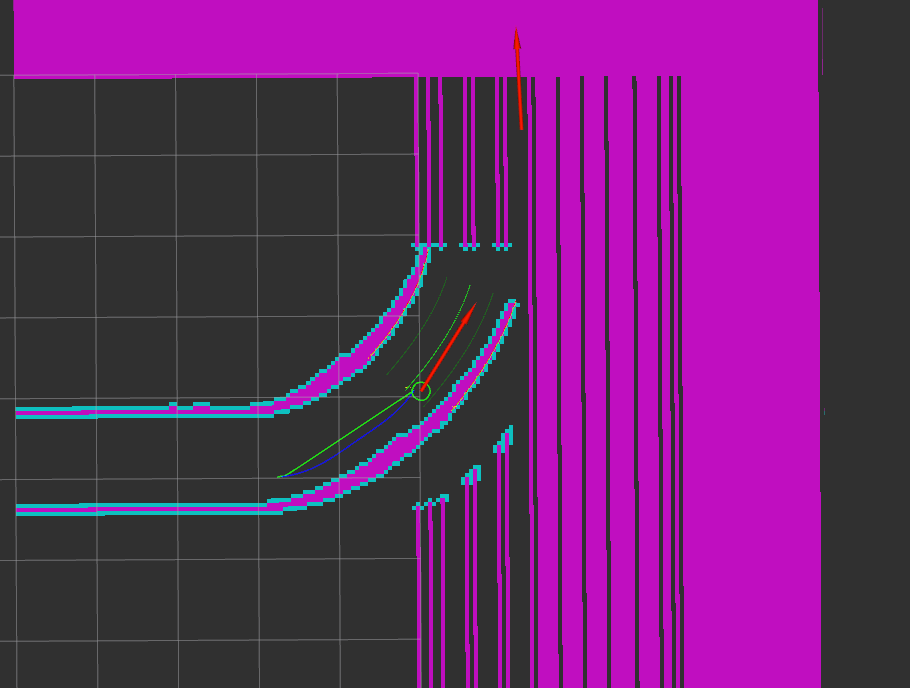
\includegraphics[width=\textwidth]{Pictures/borders}
	
	\caption{global planner border error}
	\label{boardererror}
\end{figure}

To prevent this behavior the not documented parameter ``outline\_map'' has to be set to false. The default value of this parameter is therefore changed in the forked version of the navigation stack.

To make planning easier the parameter ``cost\_factor'' can be reduced. This parameter multiplies the cost of every cell in the costmap before planning, which
 would make the gradually decreasing cost of the dynamic\_cost\_layer redundant.
 
 
 While using the global\_planner plugin a bug during the potential field calculation has been observed as pictured in \ref{potentialfield}. This bug causes an error of the planner, since it is not able to resolve a path, even though the potential field exists. Which therefore leads to the robot continuing to drive with the same velocities,  until the planner manages to construct a valid potential field again. In this moment the robot often leaves the right lane even though there is no obstacle infront of it.
 
 This bug has been reported to the developer of the plugin.
 
 \begin{figure}[H]
 	\centering
 	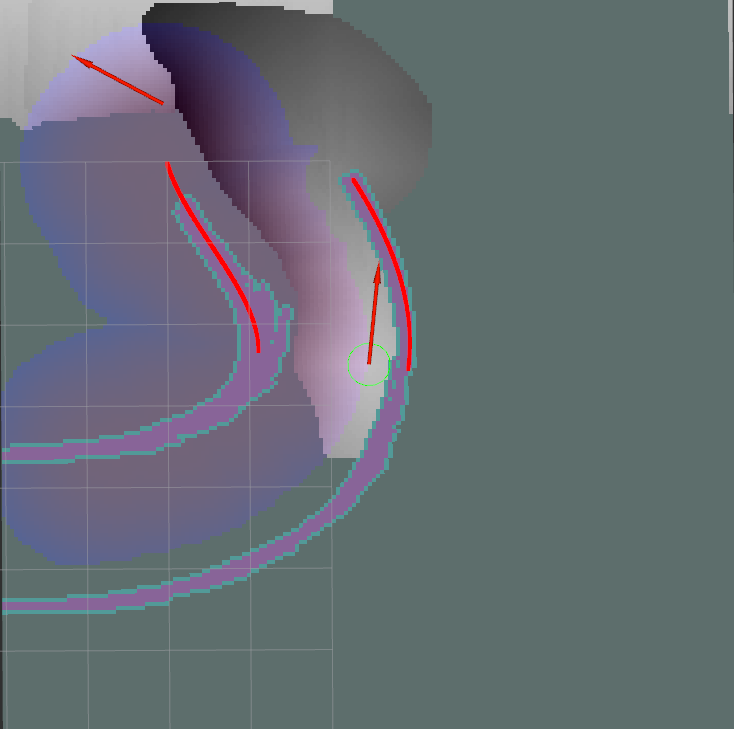
\includegraphics[width=.7\textwidth]{Pictures/out of bounds}	
 	
 	\caption{potential field generated by global\_planner plugin}
 	\label{potentialfield}
 \end{figure}


\subsection{teb\_local\_planner}

Like the global planner the local planner has to be configured to comply its tasks.

A good starting point for the configuration are the example configurations in the repository of the developer of the planner\cite{tebtutorials}. They offer base configurations for both differential drive and car like, aswell as omnidirectional robots.\\

Unfortunately teb\_local\_planner only considers lethal cost and without any configuration would follow the global path very loosely resulting in e.g. cutting corners.\\ 

To give the planner a tendency to follow the global planner closer the option ``viapoint'' can be used. This allows to set points at a configurable distance to each other on the global path, that pull the local path and the robot to the correct lane. The attraction of the local path through the via points is then tuned so the robot drives roughly in the middle of the right lane, when no obstacle is on the road, but still can separate itself from the global path, when avoiding obstacles.\\

The parameter ``max\_global\_plan\_lookahead\_dist'' controls how much of the global plan is actually considered by the local planner. This parameter highly influences the computational load when setting the distance to larger values. Using shorted distances results in oscillations while driving straight, which is caused by the jumping global path.\\

During testing teb\_local\_planner produced mostly good and feasible paths, but sometimes it generated loops along the global path, that would result in the robot turning in spot, before it follows the global path further. This leads to the robot changing the driving direction since after half of a turn the PoseFinder finds new goals, that are feasible.\\

To suppress this behavior the weighting of the time component has been increased so the internal forces that contract the elastic band increase. This reduced the occurrence of this scenario significantly, but the local path takes longer, until it is on the right lane again, since the distance to the global path is now weighted less relative to the weight of the time component.

\section{Odometry test}
The odometry is a key component in the navigation concept, since it will be used by multiple nodes and is the representation of the robots position in its environment.\\

Especially differential robots tend to have rotational error, when using the wheel-encoders to generate the odometry, since the wheels are forced to slip when the robot is turning.\\

To test the quality of the odometry the robot will be placed in the world pictured in Figure \ref{simworld}. Now the robot is supposed to drive one round, during which the odometry of the robot will be tracked.\\

In theory the trace of the odometry should be closed perfectly, after the robot performed its first round.\\

\section{Lidar test}
The lidar is the only sensor, which detects static obstacles in the surrounding of the robot. Hence the quality of the data has to be checked.

To test the performance of the simulated lidar the robot will simply navigate in the world pictured in Figure \ref{simworld} and detect obstacles along the road.\\

The quality of the data will be observed by looking at the raw data, aswell as the costmap, that receives the measurements of the lidar.\\

The evaluation of the costmap is necesarry, since it will mark measurements of the lidar as lethal. With increasing noise the marked obstacles will be less precise, therefore the lidar has direct influence on the performance of the navigation even when obstacles are not on the road.

The main focus of this test is sensor noise, since the Gazebo sensor plugin is configured based on the data sheet of the real lidar (Appendix \ref{AppendixDataSheets}).

\section{road\_detection test}
As the road\_detection is the only data source providing informations about the road it is crucial for successful navigation.

To check if the roadDetection offers good enough results a long duration test will be performed, during which the output of the roadRecordEvaluation node will be monitored, which outputs the relation between the amount of recognized road and overall attempts to find a road.\\

The robot will navigate on the course pictured in Figure \ref{simworld} until the output of the roadRecordEvaluation settles to a reliable result.

\section{SLAM test}
The SLAM algorithm chosen for the the concept is used in a very uncommon way, since it is not only receiving input from a real range finding sensor, but as well from the road detection.

The data from the road detection is very self similar, meaning that for example a straight section of road will always look very similar independent of its position. The lack of details in the data from the road detection might complicate cartographers scan matching.\\

\textbf{Data purely from road detection:}\\
The reason for this test is to check if the SLAM algorithm can handle mapping with as least information as possible. This will make loop-closure difficult and cartographer has to work with the self similar data only.\\
The aim is, that the robot can drive multiple rounds, on the track and cartographer produces an optimized map with little unmatched submaps and well connected road markings.\\

\textbf{Long duration test with both road detection and lidar scan with obstacles on the side of the road:}\\
Cartographer seems to not merge old submaps but process all of them always, which will progressively increase computational load. Since the SLAM is supposed to be used during mapping, this can become important with a lot of sensor inputs that offer constraint potential and long runtime.
The same setup as in the \nth{2} test will be used but the focus is on the moment, at which cartographer cannot optimize in real time caused by too many submaps and constraints.\\


\textbf{Data purely from localization and lidar scan with obstacles on the road:}\\
This test is meant to be the worst case for the SLAM algorithm during navigation. The purpose is to check how cartographer handles data loss during obstacle avoidance and lane swapping.
The obstacles will be placed in two corners and therefore in the edge case where the camera has the worst chance of seeing the road because of the steering angle, aswell as on the straight section of the road to cover the case where the camera can not see the road during merging on an other lane. Furthermore the obstacles will be placed far enough apart so the lidar has only vision on one at the same time.\\


\section{Complete system test}

After the previous tests the entire concept has to be tested in order to check, if the concept works as anticipated.

Autonomous navigation in the following test scenarios will be performed:

\begin{itemize}
	\item no obstacles
	\item obstacles on left lane
	\item obstacles on right lane
\end{itemize}

During all test the following criteria will be monitored aswell as any unexpected problems during the test:

\begin{itemize}
	\item distance to the right lane when no obstacle is close
	\item obstacle avoidance distance to object
\end{itemize}

For these tests the exact position of the obstacles and the robot will be used for evaluation. This allows to determine the exact distance between the robot and obstacles, aswell as if the robot is still on the road.\\
The distance to the right lane will be determined by using the polynomial provided by the road detection. A so called ``avoidance'' starts when the robot is just slightly over the middle line, without any hysteresis.

As defined in the rules of the Carolo-Cup the merging onto the right lane during the obstacle avoidance is supposed to take place within the next two meters after an obstacle \cite{carolocup}.

In all tests the robot will drive multiple rounds if possible to produce reliable results. The tests will be performed in the environment pictured in Figure \ref{simworld}.\\












